\documentclass[]{article}
\usepackage{lmodern}
\usepackage{amssymb,amsmath}
\usepackage{ifxetex,ifluatex}
\usepackage{fixltx2e} % provides \textsubscript
\ifnum 0\ifxetex 1\fi\ifluatex 1\fi=0 % if pdftex
  \usepackage[T1]{fontenc}
  \usepackage[utf8]{inputenc}
\else % if luatex or xelatex
  \ifxetex
    \usepackage{mathspec}
  \else
    \usepackage{fontspec}
  \fi
  \defaultfontfeatures{Ligatures=TeX,Scale=MatchLowercase}
\fi
% use upquote if available, for straight quotes in verbatim environments
\IfFileExists{upquote.sty}{\usepackage{upquote}}{}
% use microtype if available
\IfFileExists{microtype.sty}{%
\usepackage{microtype}
\UseMicrotypeSet[protrusion]{basicmath} % disable protrusion for tt fonts
}{}
\usepackage[margin=1in]{geometry}
\usepackage{hyperref}
\hypersetup{unicode=true,
            pdftitle={Linguistic Data: Quantitative Analysis and Visualisation},
            pdfborder={0 0 0},
            breaklinks=true}
\urlstyle{same}  % don't use monospace font for urls
\usepackage{color}
\usepackage{fancyvrb}
\newcommand{\VerbBar}{|}
\newcommand{\VERB}{\Verb[commandchars=\\\{\}]}
\DefineVerbatimEnvironment{Highlighting}{Verbatim}{commandchars=\\\{\}}
% Add ',fontsize=\small' for more characters per line
\usepackage{framed}
\definecolor{shadecolor}{RGB}{248,248,248}
\newenvironment{Shaded}{\begin{snugshade}}{\end{snugshade}}
\newcommand{\KeywordTok}[1]{\textcolor[rgb]{0.13,0.29,0.53}{\textbf{#1}}}
\newcommand{\DataTypeTok}[1]{\textcolor[rgb]{0.13,0.29,0.53}{#1}}
\newcommand{\DecValTok}[1]{\textcolor[rgb]{0.00,0.00,0.81}{#1}}
\newcommand{\BaseNTok}[1]{\textcolor[rgb]{0.00,0.00,0.81}{#1}}
\newcommand{\FloatTok}[1]{\textcolor[rgb]{0.00,0.00,0.81}{#1}}
\newcommand{\ConstantTok}[1]{\textcolor[rgb]{0.00,0.00,0.00}{#1}}
\newcommand{\CharTok}[1]{\textcolor[rgb]{0.31,0.60,0.02}{#1}}
\newcommand{\SpecialCharTok}[1]{\textcolor[rgb]{0.00,0.00,0.00}{#1}}
\newcommand{\StringTok}[1]{\textcolor[rgb]{0.31,0.60,0.02}{#1}}
\newcommand{\VerbatimStringTok}[1]{\textcolor[rgb]{0.31,0.60,0.02}{#1}}
\newcommand{\SpecialStringTok}[1]{\textcolor[rgb]{0.31,0.60,0.02}{#1}}
\newcommand{\ImportTok}[1]{#1}
\newcommand{\CommentTok}[1]{\textcolor[rgb]{0.56,0.35,0.01}{\textit{#1}}}
\newcommand{\DocumentationTok}[1]{\textcolor[rgb]{0.56,0.35,0.01}{\textbf{\textit{#1}}}}
\newcommand{\AnnotationTok}[1]{\textcolor[rgb]{0.56,0.35,0.01}{\textbf{\textit{#1}}}}
\newcommand{\CommentVarTok}[1]{\textcolor[rgb]{0.56,0.35,0.01}{\textbf{\textit{#1}}}}
\newcommand{\OtherTok}[1]{\textcolor[rgb]{0.56,0.35,0.01}{#1}}
\newcommand{\FunctionTok}[1]{\textcolor[rgb]{0.00,0.00,0.00}{#1}}
\newcommand{\VariableTok}[1]{\textcolor[rgb]{0.00,0.00,0.00}{#1}}
\newcommand{\ControlFlowTok}[1]{\textcolor[rgb]{0.13,0.29,0.53}{\textbf{#1}}}
\newcommand{\OperatorTok}[1]{\textcolor[rgb]{0.81,0.36,0.00}{\textbf{#1}}}
\newcommand{\BuiltInTok}[1]{#1}
\newcommand{\ExtensionTok}[1]{#1}
\newcommand{\PreprocessorTok}[1]{\textcolor[rgb]{0.56,0.35,0.01}{\textit{#1}}}
\newcommand{\AttributeTok}[1]{\textcolor[rgb]{0.77,0.63,0.00}{#1}}
\newcommand{\RegionMarkerTok}[1]{#1}
\newcommand{\InformationTok}[1]{\textcolor[rgb]{0.56,0.35,0.01}{\textbf{\textit{#1}}}}
\newcommand{\WarningTok}[1]{\textcolor[rgb]{0.56,0.35,0.01}{\textbf{\textit{#1}}}}
\newcommand{\AlertTok}[1]{\textcolor[rgb]{0.94,0.16,0.16}{#1}}
\newcommand{\ErrorTok}[1]{\textcolor[rgb]{0.64,0.00,0.00}{\textbf{#1}}}
\newcommand{\NormalTok}[1]{#1}
\usepackage{graphicx,grffile}
\makeatletter
\def\maxwidth{\ifdim\Gin@nat@width>\linewidth\linewidth\else\Gin@nat@width\fi}
\def\maxheight{\ifdim\Gin@nat@height>\textheight\textheight\else\Gin@nat@height\fi}
\makeatother
% Scale images if necessary, so that they will not overflow the page
% margins by default, and it is still possible to overwrite the defaults
% using explicit options in \includegraphics[width, height, ...]{}
\setkeys{Gin}{width=\maxwidth,height=\maxheight,keepaspectratio}
\IfFileExists{parskip.sty}{%
\usepackage{parskip}
}{% else
\setlength{\parindent}{0pt}
\setlength{\parskip}{6pt plus 2pt minus 1pt}
}
\setlength{\emergencystretch}{3em}  % prevent overfull lines
\providecommand{\tightlist}{%
  \setlength{\itemsep}{0pt}\setlength{\parskip}{0pt}}
\setcounter{secnumdepth}{0}
% Redefines (sub)paragraphs to behave more like sections
\ifx\paragraph\undefined\else
\let\oldparagraph\paragraph
\renewcommand{\paragraph}[1]{\oldparagraph{#1}\mbox{}}
\fi
\ifx\subparagraph\undefined\else
\let\oldsubparagraph\subparagraph
\renewcommand{\subparagraph}[1]{\oldsubparagraph{#1}\mbox{}}
\fi

%%% Use protect on footnotes to avoid problems with footnotes in titles
\let\rmarkdownfootnote\footnote%
\def\footnote{\protect\rmarkdownfootnote}

%%% Change title format to be more compact
\usepackage{titling}

% Create subtitle command for use in maketitle
\newcommand{\subtitle}[1]{
  \posttitle{
    \begin{center}\large#1\end{center}
    }
}

\setlength{\droptitle}{-2em}

  \title{Linguistic Data: Quantitative Analysis and Visualisation}
    \pretitle{\vspace{\droptitle}\centering\huge}
  \posttitle{\par}
  \subtitle{Lab on a Student's t-test}
  \author{}
    \preauthor{}\postauthor{}
    \date{}
    \predate{}\postdate{}
  

\begin{document}
\maketitle

\subsubsection{Aspiration and vowel duration in
Icelandic}\label{aspiration-and-vowel-duration-in-icelandic}

This set is based on (Coretta 2017, \href{https://goo.gl/NrfgJm}{link}.
This dissertation dealt with the relation between vowel duration and
aspiration in consonants. Author carried out a data collection with 5
natives speakers of Icelandic. Then he extracted the duration of vowels
followed by aspirated versus non-aspirated consonants. Check out whether
vowels before aspirated consonants (like in Icelandic takka `key'
{[}tʰaʰka{]}) are significantly shorter than vowels followed by
non-aspirated consonants (like in kagga `barrel' {[}kʰakka{]}).
\href{http://math-info.hse.ru/f/2018-19/ling-data/icelandic.csv}{Link}
to the dataset.

\begin{Shaded}
\begin{Highlighting}[]
\NormalTok{df <-}\StringTok{ }\KeywordTok{read.csv}\NormalTok{(}\StringTok{"http://math-info.hse.ru/f/2018-19/ling-data/icelandic.csv"}\NormalTok{)}
\end{Highlighting}
\end{Shaded}

\subsubsection{Descriptive statistics}\label{descriptive-statistics}

A general boxplot:

\begin{Shaded}
\begin{Highlighting}[]
\KeywordTok{boxplot}\NormalTok{(df}\OperatorTok{$}\NormalTok{vowel.dur)}
\end{Highlighting}
\end{Shaded}

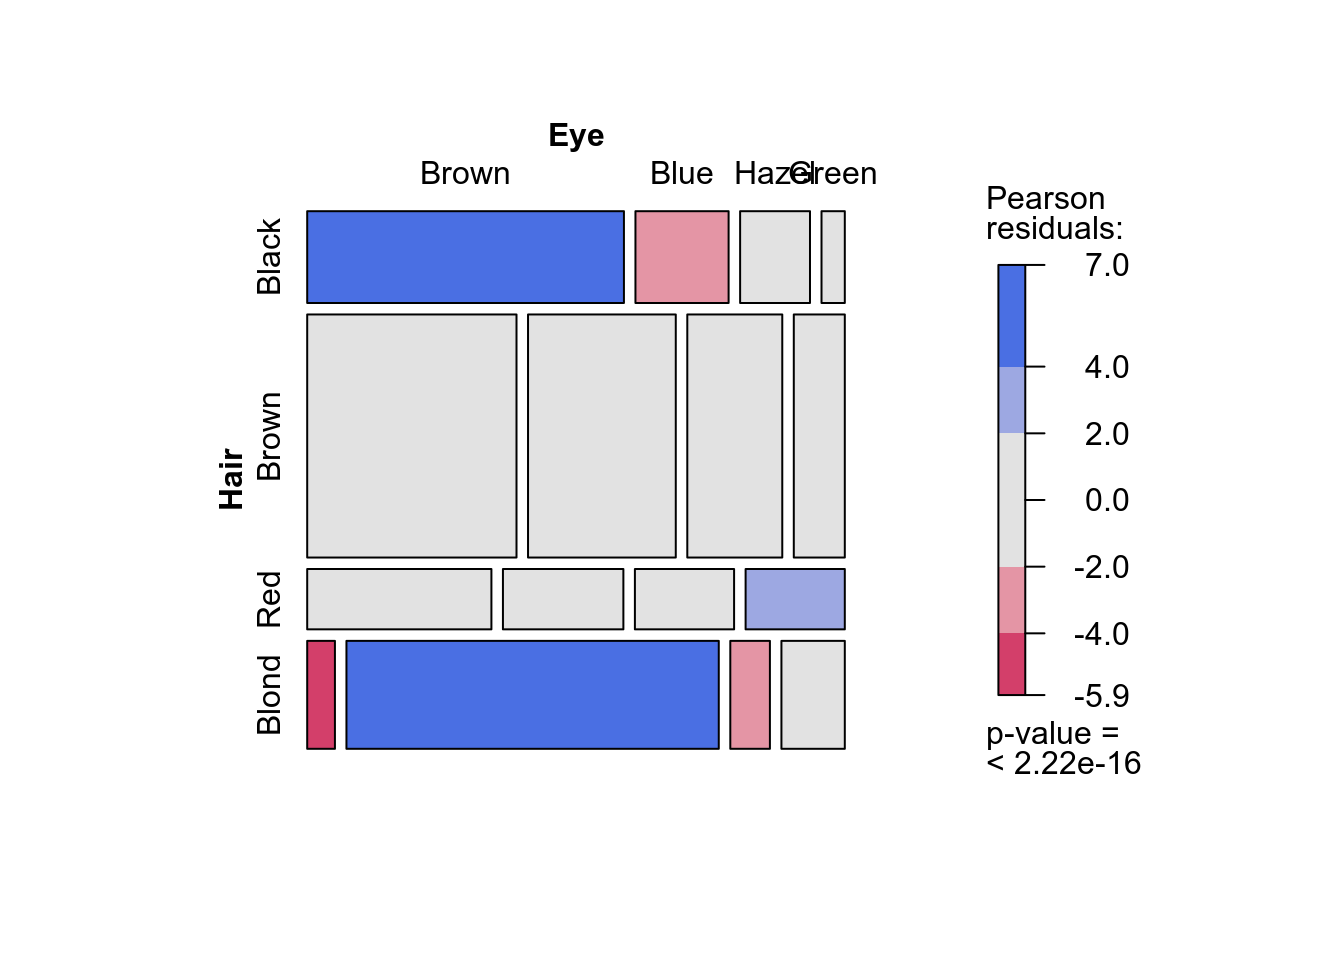
\includegraphics{LingData-Lab4-comp_files/figure-latex/unnamed-chunk-2-1.pdf}

Get the number of outliers:

\begin{Shaded}
\begin{Highlighting}[]
\KeywordTok{length}\NormalTok{(}\KeywordTok{boxplot}\NormalTok{(df}\OperatorTok{$}\NormalTok{vowel.dur)}\OperatorTok{$}\NormalTok{out)}
\end{Highlighting}
\end{Shaded}

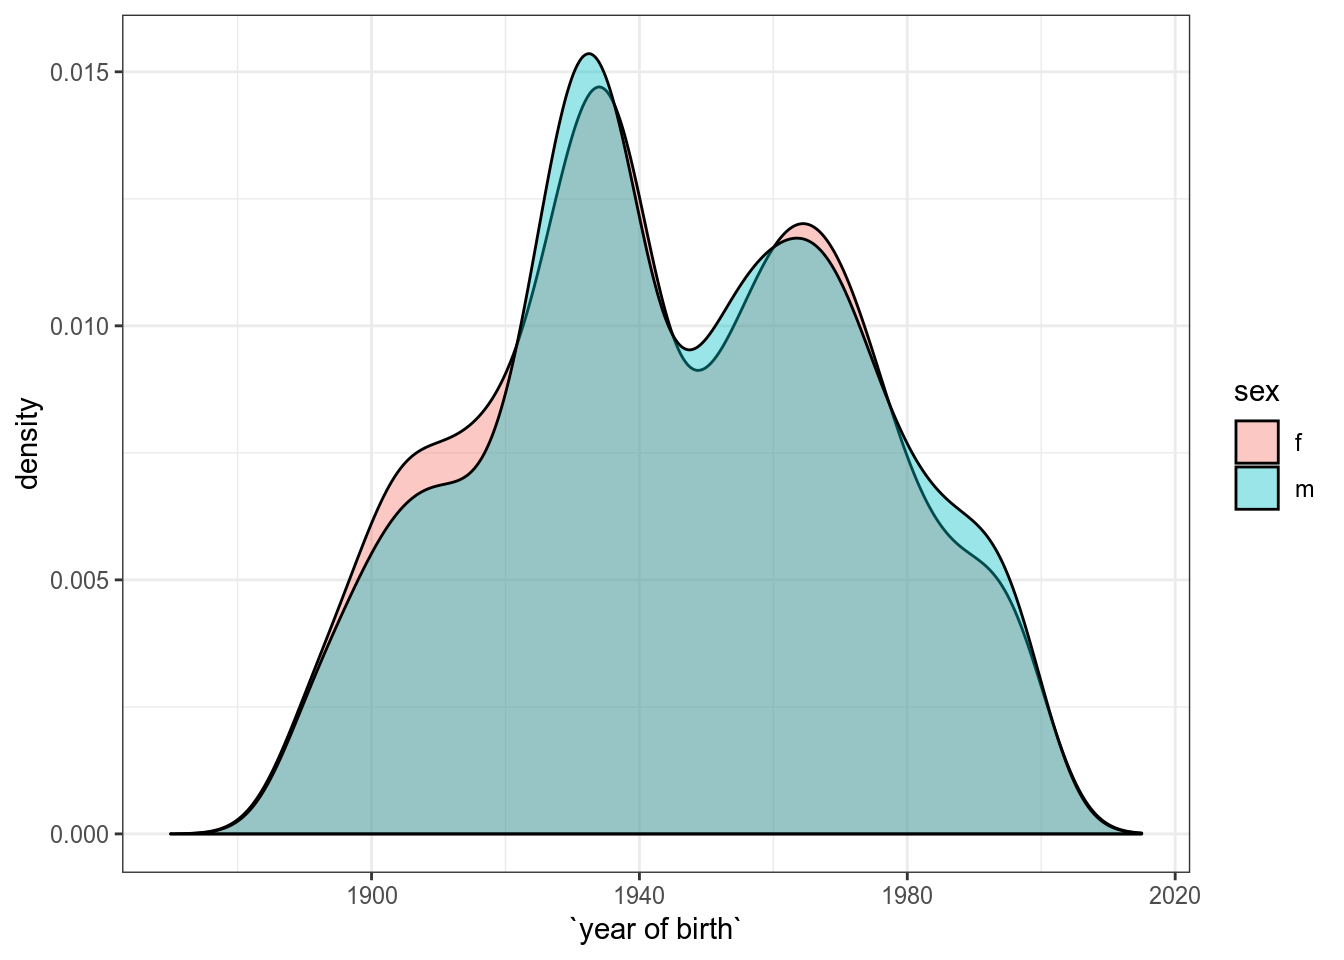
\includegraphics{LingData-Lab4-comp_files/figure-latex/unnamed-chunk-3-1.pdf}

\begin{verbatim}
## [1] 27
\end{verbatim}

Look at number of observations by groups (aspirated and non-aspirated
cases):

\begin{Shaded}
\begin{Highlighting}[]
\KeywordTok{table}\NormalTok{(df}\OperatorTok{$}\NormalTok{aspriration)}
\end{Highlighting}
\end{Shaded}

\begin{verbatim}
## < table of extent 0 >
\end{verbatim}

Choose two subsamples, one for words where vowels are followed by
aspirated consonants and another for non-aspirated consonants.

\begin{Shaded}
\begin{Highlighting}[]
\NormalTok{asp <-}\StringTok{ }\NormalTok{df[df}\OperatorTok{$}\NormalTok{aspiration }\OperatorTok{==}\StringTok{ 'yes'}\NormalTok{,]}
\NormalTok{nasp <-}\StringTok{ }\NormalTok{df[df}\OperatorTok{$}\NormalTok{aspiration }\OperatorTok{==}\StringTok{ 'no'}\NormalTok{,]}
\end{Highlighting}
\end{Shaded}

Summary for aspirated and non-aspirated cases:

\begin{Shaded}
\begin{Highlighting}[]
\KeywordTok{summary}\NormalTok{(asp}\OperatorTok{$}\NormalTok{vowel.dur)}
\end{Highlighting}
\end{Shaded}

\begin{verbatim}
##    Min. 1st Qu.  Median    Mean 3rd Qu.    Max. 
##   22.78   64.96   77.60   78.76   91.46  166.56
\end{verbatim}

\begin{Shaded}
\begin{Highlighting}[]
\KeywordTok{summary}\NormalTok{(nasp}\OperatorTok{$}\NormalTok{vowel.dur)}
\end{Highlighting}
\end{Shaded}

\begin{verbatim}
##    Min. 1st Qu.  Median    Mean 3rd Qu.    Max. 
##   37.98   77.56   91.91   94.69  103.88  214.48
\end{verbatim}

Boxplot by groups:

\begin{Shaded}
\begin{Highlighting}[]
\KeywordTok{boxplot}\NormalTok{(df}\OperatorTok{$}\NormalTok{vowel.dur }\OperatorTok{~}\StringTok{ }\NormalTok{df}\OperatorTok{$}\NormalTok{aspiration)}
\end{Highlighting}
\end{Shaded}

\includegraphics{LingData-Lab4-comp_files/figure-latex/unnamed-chunk-7-1.pdf}

More interesting - let us create a boxplot by all groups (see the field
\texttt{cons1}):

\begin{Shaded}
\begin{Highlighting}[]
\KeywordTok{boxplot}\NormalTok{(df}\OperatorTok{$}\NormalTok{vowel.dur }\OperatorTok{~}\StringTok{ }\NormalTok{df}\OperatorTok{$}\NormalTok{cons1)}
\end{Highlighting}
\end{Shaded}

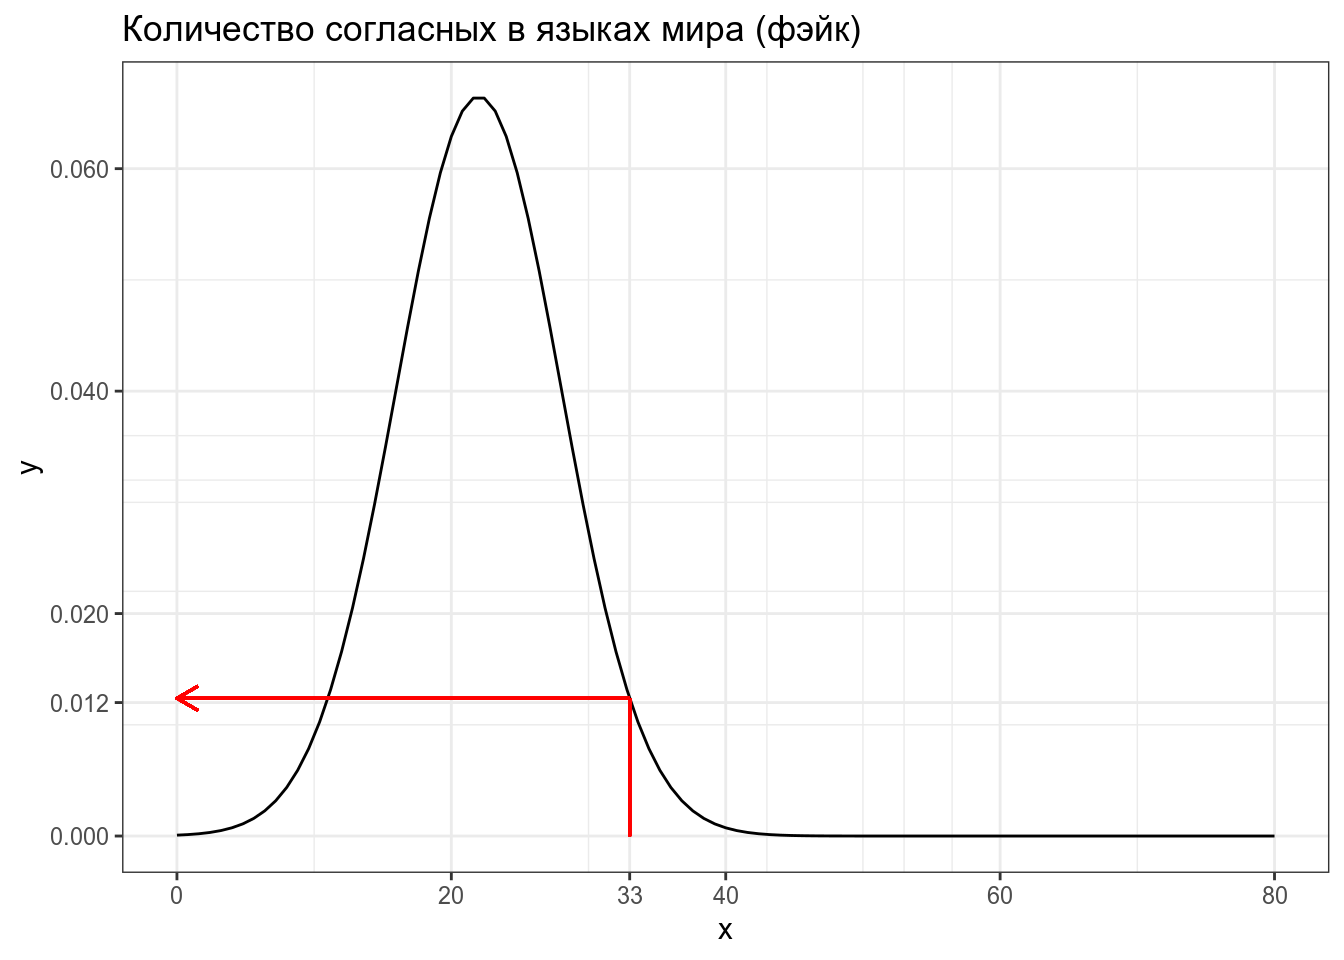
\includegraphics{LingData-Lab4-comp_files/figure-latex/unnamed-chunk-8-1.pdf}

You can compare distribution of \texttt{vowel.dur} in asp(irated),
fri(cative), nasp(non-aspirated), voi(ced), etc.

We can limit our data to just one type of vowels, say, middle vowels.
Therefore, we will work with the same type of a consonant:

\begin{Shaded}
\begin{Highlighting}[]
\NormalTok{asp <-}\StringTok{ }\NormalTok{df[df}\OperatorTok{$}\NormalTok{aspiration }\OperatorTok{==}\StringTok{ 'yes'} \OperatorTok{&}\StringTok{ }\NormalTok{df}\OperatorTok{$}\NormalTok{height }\OperatorTok{==}\StringTok{ 'mid'}\NormalTok{, ]}
\NormalTok{nasp <-}\StringTok{ }\NormalTok{df[df}\OperatorTok{$}\NormalTok{aspiration }\OperatorTok{==}\StringTok{ 'no'} \OperatorTok{&}\StringTok{ }\NormalTok{df}\OperatorTok{$}\NormalTok{height }\OperatorTok{==}\StringTok{ 'mid'}\NormalTok{, ]}
\end{Highlighting}
\end{Shaded}

Again, here is a summary for a corrected case:

\begin{Shaded}
\begin{Highlighting}[]
\KeywordTok{summary}\NormalTok{(asp}\OperatorTok{$}\NormalTok{vowel.dur)}
\end{Highlighting}
\end{Shaded}

\begin{verbatim}
##    Min. 1st Qu.  Median    Mean 3rd Qu.    Max. 
##   38.67   71.41   81.92   82.65   95.19  150.46
\end{verbatim}

\begin{Shaded}
\begin{Highlighting}[]
\KeywordTok{summary}\NormalTok{(nasp}\OperatorTok{$}\NormalTok{vowel.dur)}
\end{Highlighting}
\end{Shaded}

\begin{verbatim}
##    Min. 1st Qu.  Median    Mean 3rd Qu.    Max. 
##   37.98   80.90   97.97   98.73  110.51  190.93
\end{verbatim}

\begin{Shaded}
\begin{Highlighting}[]
\KeywordTok{nrow}\NormalTok{(asp)}
\end{Highlighting}
\end{Shaded}

\begin{verbatim}
## [1] 156
\end{verbatim}

\begin{Shaded}
\begin{Highlighting}[]
\KeywordTok{nrow}\NormalTok{(nasp)}
\end{Highlighting}
\end{Shaded}

\begin{verbatim}
## [1] 174
\end{verbatim}

\subsubsection{T-test}\label{t-test}

Let us formulate the null hypothesis, the alternative hypotesis, and
apply t-test to our dataset.

\begin{Shaded}
\begin{Highlighting}[]
\KeywordTok{t.test}\NormalTok{(asp}\OperatorTok{$}\NormalTok{vowel.dur, nasp}\OperatorTok{$}\NormalTok{vowel.dur)}
\end{Highlighting}
\end{Shaded}

\begin{verbatim}
## 
##  Welch Two Sample t-test
## 
## data:  asp$vowel.dur and nasp$vowel.dur
## t = -6.4869, df = 317.72, p-value = 3.356e-10
## alternative hypothesis: true difference in means is not equal to 0
## 95 percent confidence interval:
##  -20.94772 -11.19801
## sample estimates:
## mean of x mean of y 
##  82.65371  98.72657
\end{verbatim}

By default, R calculates t.test with regard to the bi-directional
alternative hypothesis, such as \(\mu_1 \neq \mu_2\).

\subsubsection{Unidirectional t-test}\label{unidirectional-t-test}

H1: \(\mu_{asp} \lt \mu_{nasp}\)

\begin{Shaded}
\begin{Highlighting}[]
\KeywordTok{t.test}\NormalTok{(asp}\OperatorTok{$}\NormalTok{vowel.dur, nasp}\OperatorTok{$}\NormalTok{vowel.dur, }\DataTypeTok{alternative =} \StringTok{"less"}\NormalTok{)}
\end{Highlighting}
\end{Shaded}

\begin{verbatim}
## 
##  Welch Two Sample t-test
## 
## data:  asp$vowel.dur and nasp$vowel.dur
## t = -6.4869, df = 317.72, p-value = 1.678e-10
## alternative hypothesis: true difference in means is less than 0
## 95 percent confidence interval:
##       -Inf -11.98542
## sample estimates:
## mean of x mean of y 
##  82.65371  98.72657
\end{verbatim}

\subsubsection{Density plots}\label{density-plots}

\begin{Shaded}
\begin{Highlighting}[]
\KeywordTok{require}\NormalTok{(tidyverse)}
\end{Highlighting}
\end{Shaded}

\begin{verbatim}
## Loading required package: tidyverse
\end{verbatim}

\begin{verbatim}
## Warning in library(package, lib.loc = lib.loc, character.only = TRUE,
## logical.return = TRUE, : there is no package called 'tidyverse'
\end{verbatim}

\begin{Shaded}
\begin{Highlighting}[]
\KeywordTok{require}\NormalTok{(dplyr)}
\end{Highlighting}
\end{Shaded}

\begin{verbatim}
## Loading required package: dplyr
\end{verbatim}

\begin{verbatim}
## 
## Attaching package: 'dplyr'
\end{verbatim}

\begin{verbatim}
## The following objects are masked from 'package:stats':
## 
##     filter, lag
\end{verbatim}

\begin{verbatim}
## The following objects are masked from 'package:base':
## 
##     intersect, setdiff, setequal, union
\end{verbatim}

Let's get a descriptive summary of our data in a dplyr style.

\begin{Shaded}
\begin{Highlighting}[]
\NormalTok{df }\OperatorTok\StringTok{ }
\StringTok{  }\KeywordTok{group_by}\NormalTok{(aspiration) }\OperatorTok
\StringTok{  }\KeywordTok{summarise}\NormalTok{(}\DataTypeTok{mean =} \KeywordTok{mean}\NormalTok{(vowel.dur),}
            \DataTypeTok{st.dev =} \KeywordTok{sd}\NormalTok{(vowel.dur))}
\end{Highlighting}
\end{Shaded}

\begin{verbatim}
## # A tibble: 2 x 3
##   aspiration  mean st.dev
##   <fct>      <dbl>  <dbl>
## 1 no          94.7   25.9
## 2 yes         78.8   21.2
\end{verbatim}

Density plots can be thought of as plots of smoothed histograms.

\begin{Shaded}
\begin{Highlighting}[]
\KeywordTok{library}\NormalTok{(ggplot2)}
\NormalTok{df }\OperatorTok\StringTok{ }
\StringTok{  }\KeywordTok{ggplot}\NormalTok{(}\KeywordTok{aes}\NormalTok{(vowel.dur, }\DataTypeTok{fill =}\NormalTok{ aspiration, }\DataTypeTok{color =}\NormalTok{ aspiration))}\OperatorTok{+}
\StringTok{  }\KeywordTok{geom_density}\NormalTok{(}\DataTypeTok{alpha =} \FloatTok{0.4}\NormalTok{)}\OperatorTok{+}
\StringTok{  }\KeywordTok{geom_rug}\NormalTok{()}\OperatorTok{+}
\StringTok{  }\KeywordTok{labs}\NormalTok{(}\DataTypeTok{title =} \StringTok{"Vowel duration density plot"}\NormalTok{,}
       \DataTypeTok{caption =} \StringTok{"Data from (Coretta 2017)"}\NormalTok{,}
       \DataTypeTok{x =} \StringTok{"vowel duration"}\NormalTok{)}
\end{Highlighting}
\end{Shaded}

\includegraphics{LingData-Lab4-comp_files/figure-latex/unnamed-chunk-15-1.pdf}

Density plot by speaker:

\begin{Shaded}
\begin{Highlighting}[]
\NormalTok{df }\OperatorTok\StringTok{ }
\StringTok{  }\KeywordTok{ggplot}\NormalTok{(}\KeywordTok{aes}\NormalTok{(vowel.dur, }\DataTypeTok{fill =}\NormalTok{ aspiration, }\DataTypeTok{color =}\NormalTok{ aspiration))}\OperatorTok{+}
\StringTok{  }\KeywordTok{geom_density}\NormalTok{(}\DataTypeTok{alpha =} \FloatTok{0.4}\NormalTok{)}\OperatorTok{+}
\StringTok{  }\KeywordTok{geom_rug}\NormalTok{()}\OperatorTok{+}
\StringTok{  }\KeywordTok{facet_wrap}\NormalTok{(}\OperatorTok{~}\NormalTok{speaker)}\OperatorTok{+}
\StringTok{  }\KeywordTok{labs}\NormalTok{(}\DataTypeTok{title =} \StringTok{"Vowel duration density plot, by speaker"}\NormalTok{,}
       \DataTypeTok{caption =} \StringTok{"Data from (Coretta 2017)"}\NormalTok{,}
       \DataTypeTok{x =} \StringTok{"vowel duration"}\NormalTok{)}
\end{Highlighting}
\end{Shaded}

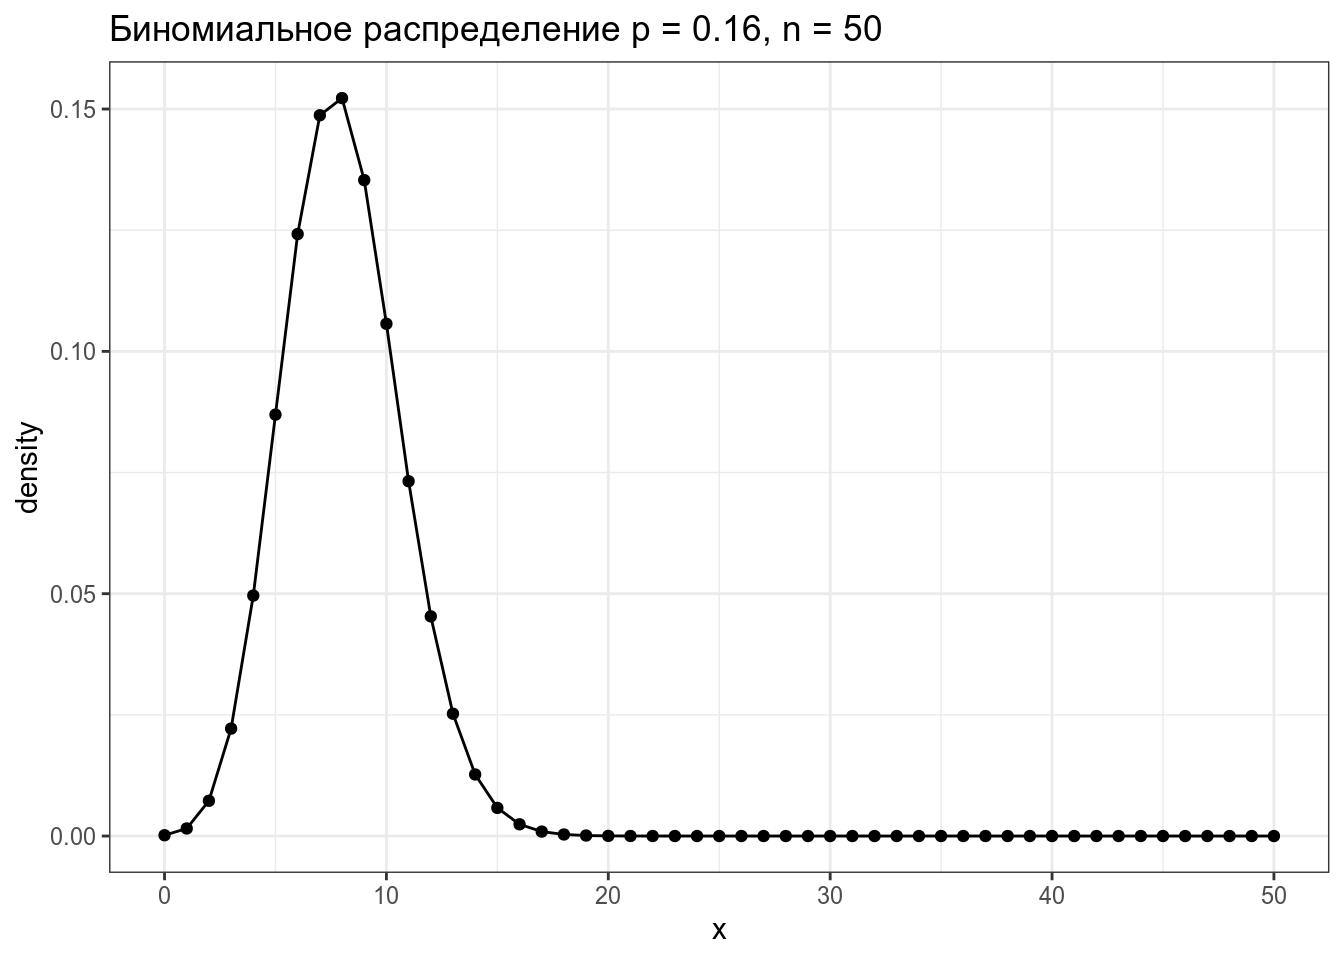
\includegraphics{LingData-Lab4-comp_files/figure-latex/unnamed-chunk-16-1.pdf}

and descriptive statistics:

\begin{Shaded}
\begin{Highlighting}[]
\NormalTok{df }\OperatorTok\StringTok{ }
\StringTok{  }\KeywordTok{group_by}\NormalTok{(aspiration, speaker) }\OperatorTok
\StringTok{  }\KeywordTok{summarise}\NormalTok{(}\DataTypeTok{mean =} \KeywordTok{mean}\NormalTok{(vowel.dur),}
            \DataTypeTok{st.dev =} \KeywordTok{sd}\NormalTok{(vowel.dur))}
\end{Highlighting}
\end{Shaded}

\begin{verbatim}
## # A tibble: 10 x 4
## # Groups:   aspiration [?]
##    aspiration speaker  mean st.dev
##    <fct>      <fct>   <dbl>  <dbl>
##  1 no         brs02    95.3   19.8
##  2 no         bte03   103.    29.4
##  3 no         jj04     95.7   25.1
##  4 no         shg05    77.7   18.9
##  5 no         tt01    101.    26.8
##  6 yes        brs02    72.9   18.9
##  7 yes        bte03    95.4   20.0
##  8 yes        jj04     86.8   20.1
##  9 yes        shg05    63.3   15.7
## 10 yes        tt01     78.3   16.7
\end{verbatim}


\end{document}
